\begin{myex}
	Ces deux graphiques représentent deux séries de même effectif et de de même moyenne $\bar{x} = 11$.
	
	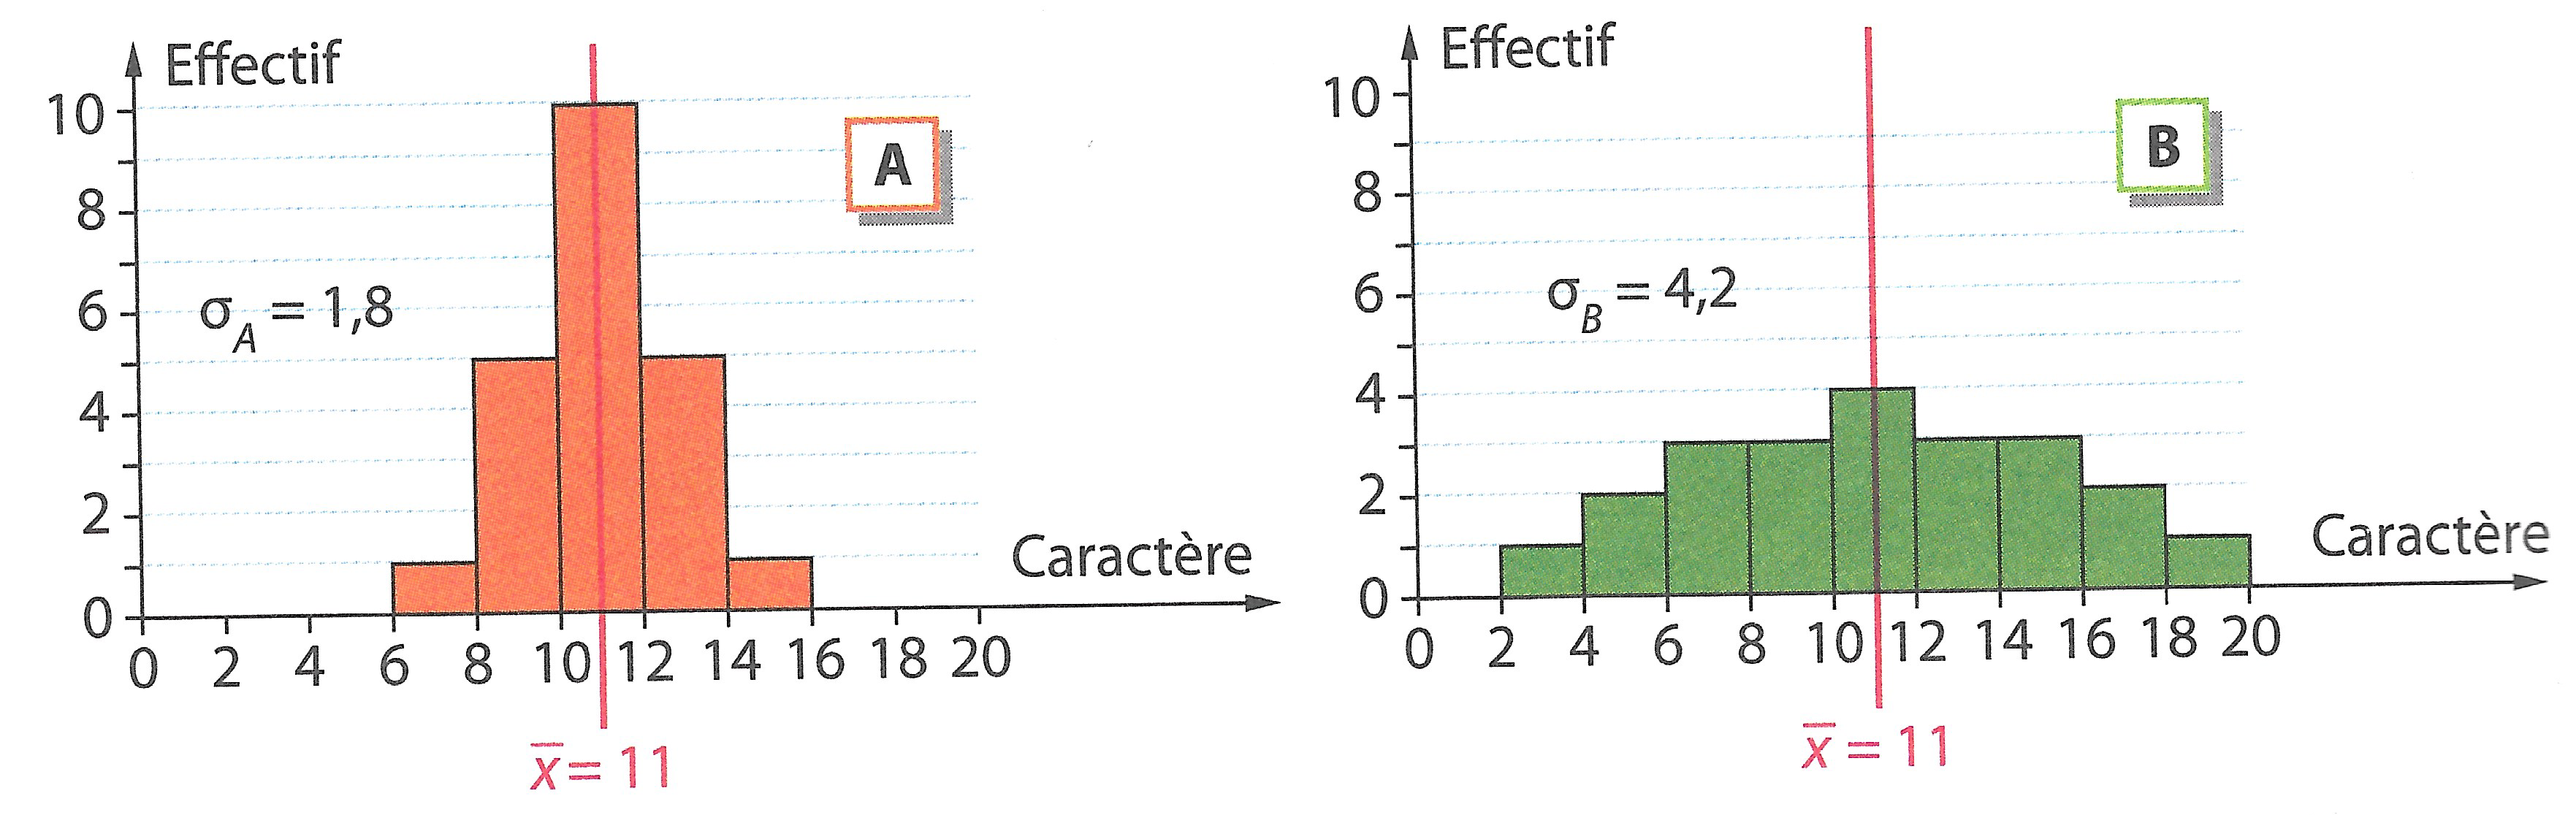
\includegraphics[scale=0.9, angle=-1.1, origin=c]{img/ex_ecart_type}
	
	$\sigma _A < \sigma _B$ : les valeurs de la série $\mathbf{B}$ sont plus dispersées que celles de la série $\mathbf{A}$ autour de $\bar{x}$. 
\end{myex}